\documentclass[11pt]{article}

\usepackage[margin=0.85in]{geometry}
\usepackage[T1]{fontenc}
\usepackage[utf8]{inputenc}
\usepackage{lmodern}
\usepackage{microtype}
\usepackage{graphicx}
\usepackage{booktabs}
\usepackage{amsmath}
\usepackage{hyperref}
\usepackage{caption}
\usepackage{float}

\hypersetup{
  colorlinks=true,
  linkcolor=blue,
  citecolor=blue,
  urlcolor=blue
}

\newcommand{\repo}{/home/lachlan/ProjectsLFS/OrganoidAgent}
\newcommand{\outroot}{/home/lachlan/ProjectsLFS/OrganoidAgent/analysis-outputs/yichao_future_expression}

\title{\textbf{Yichao Strong B2F Progress Report: Diagnosis, Correction, and Active Retraining}}
\author{OrganoidAgent Yichao analysis}
\date{May 11, 2026}

\begin{document}
\maketitle

\begin{abstract}
This report summarizes the current strong B2F training status. The first long 384 px run did not solve the task: it reached epoch 47, then stopped at the next epoch with a PyTorch activation/runtime error. More importantly, validation metrics were flat from epoch 1 through epoch 45, and prediction panels showed broad green brightfield-like outputs rather than sparse fluorescence. The cause was not simply insufficient epoch count. The training objective was encouraging a low-threshold all-signal solution, and the channels-last/SiLU path was unstable. The code has been corrected and a second 384 px long run has been started in tmux.
\end{abstract}

\section{Current Status}

\begin{table}[H]
\centering
\caption{Strong B2F run status as of this report.}
\begin{tabular}{lll}
\toprule
Run & Output folder & Status \\
\midrule
v1 strong B2F & \texttt{stage1\_b2f\_strong\_384\_long} & Stopped after epoch 47 \\
v2 corrected strong B2F & \texttt{stage1\_b2f\_strong\_384\_v2\_long} & Active in tmux \\
\bottomrule
\end{tabular}
\end{table}

The active session is:

\begin{center}
\small
\texttt{tmux attach -t yichao\_b2f\_strong\_v2}
\end{center}

The active v2 output folder is:

\begin{center}
\small
\path{/home/lachlan/ProjectsLFS/OrganoidAgent/analysis-outputs/yichao_future_expression/stage1_b2f_strong_384_v2_long}
\end{center}

\section{v1 Quantification}

The v1 run logged 47 epochs and validated every 5 epochs. The last completed validation was epoch 45.

\begin{table}[H]
\centering
\caption{v1 first and last validation metrics. Identical validation metrics show that the run was effectively stuck.}
\begin{tabular}{lcc}
\toprule
Metric & Epoch 1 & Epoch 45 \\
\midrule
Validation loss & 0.9712 & 0.9712 \\
Image MAE & 0.4173 & 0.4173 \\
Image MSE & 0.1804 & 0.1804 \\
Image PSNR & 7.44 dB & 7.44 dB \\
Masked MAE & 0.3979 & 0.3979 \\
Signal MAE & 0.3657 & 0.3657 \\
Background MAE & 0.4336 & 0.4336 \\
Signal IoU & 0.7129 & 0.7129 \\
Signal precision & 0.7129 & 0.7129 \\
Signal recall & 1.0000 & 1.0000 \\
Signal F1 & 0.8324 & 0.8324 \\
Expression AUROC & 0.3705 & 0.3705 \\
Peak Pearson & -0.2517 & -0.2517 \\
\bottomrule
\end{tabular}
\end{table}

\begin{figure}[H]
\centering
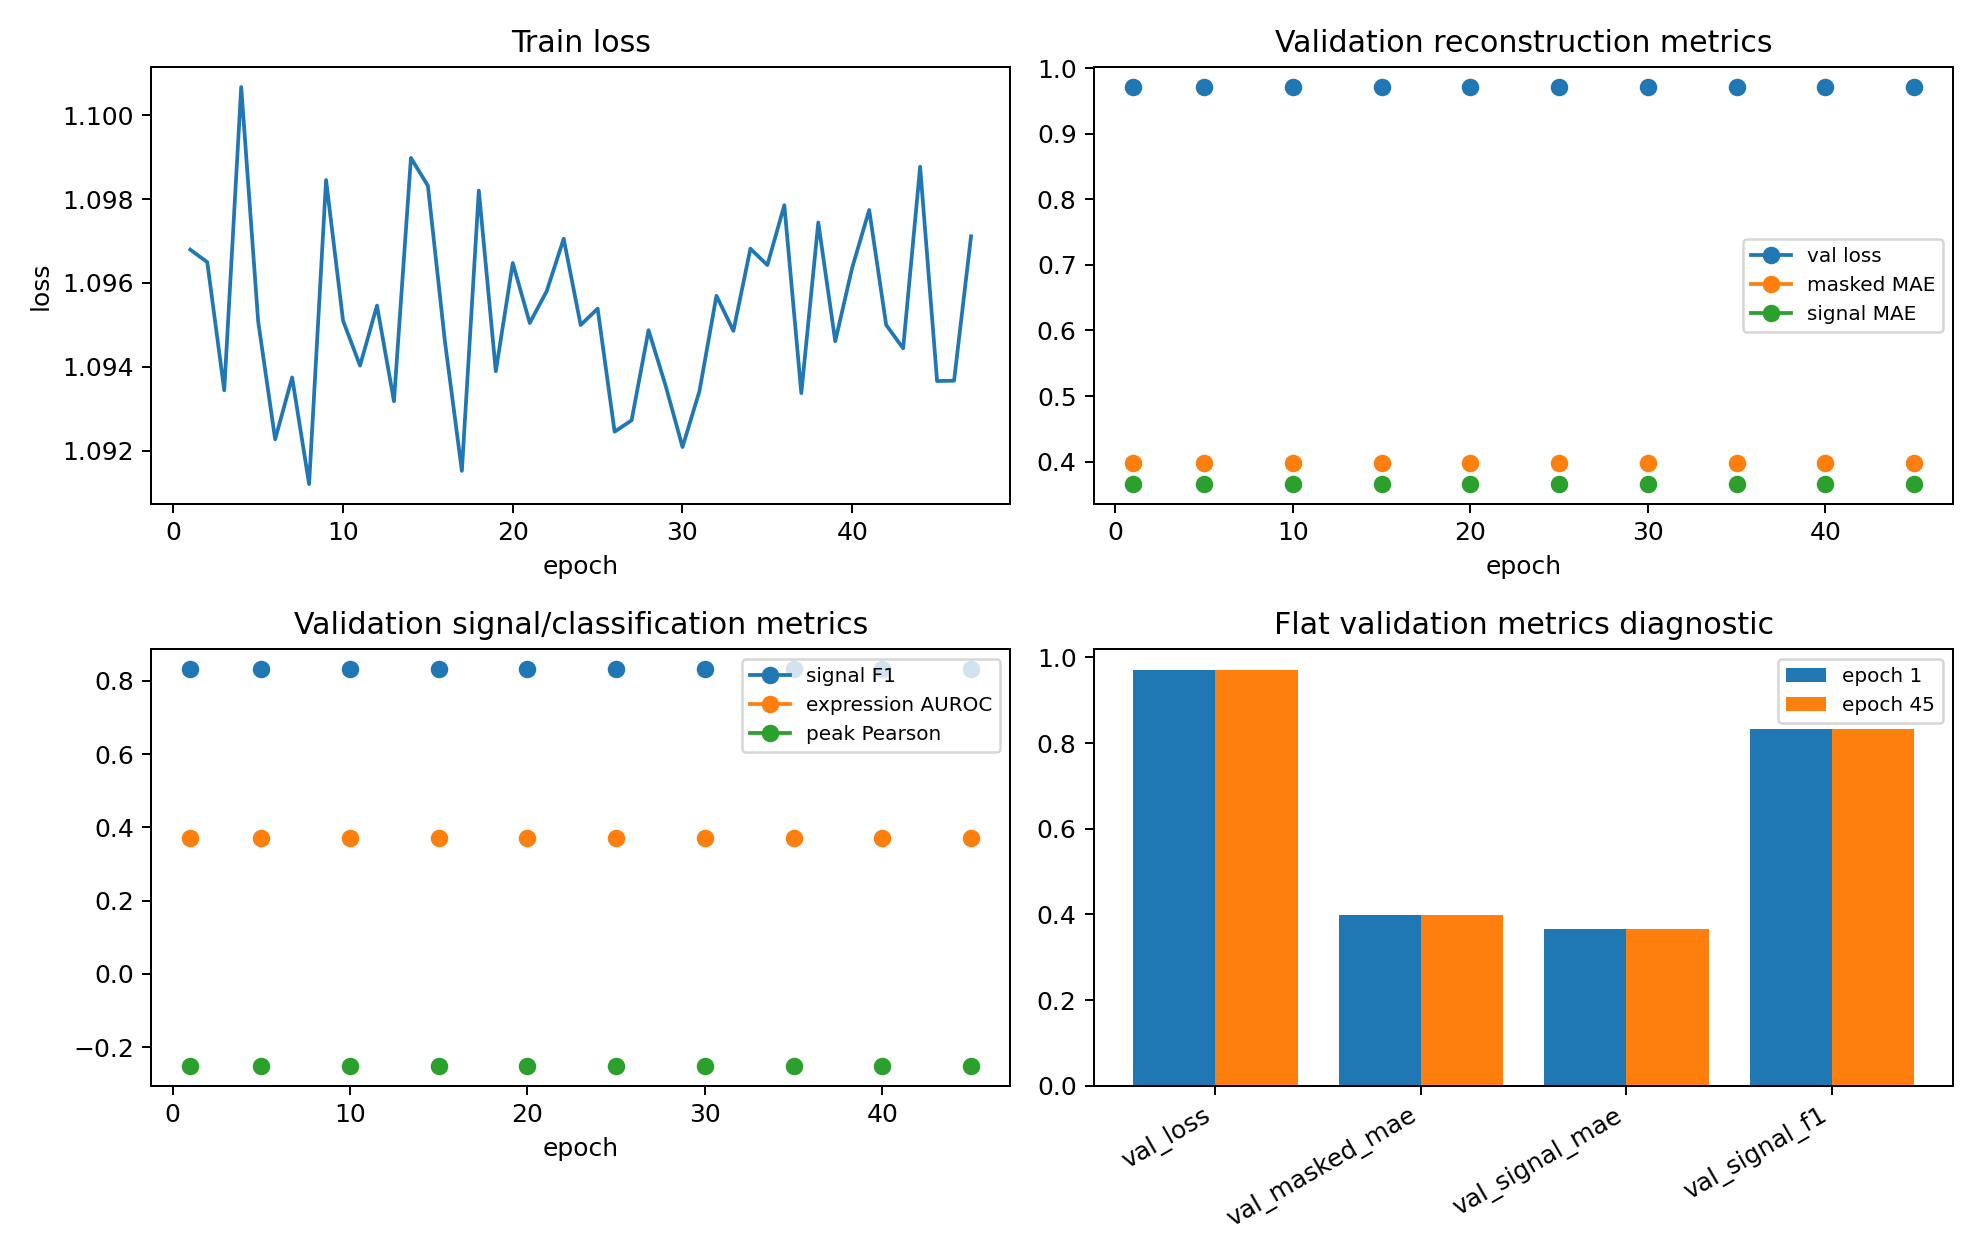
\includegraphics[width=\linewidth]{figures/fig1_v1_diagnostic_metrics.png}
\caption{v1 diagnostic metrics. Training loss fluctuated, but validation reconstruction and signal metrics were flat. This indicates a training objective/configuration problem rather than a need for more epochs.}
\label{fig:v1-metrics}
\end{figure}

\section{v1 Visual Diagnosis}

\begin{figure}[H]
\centering
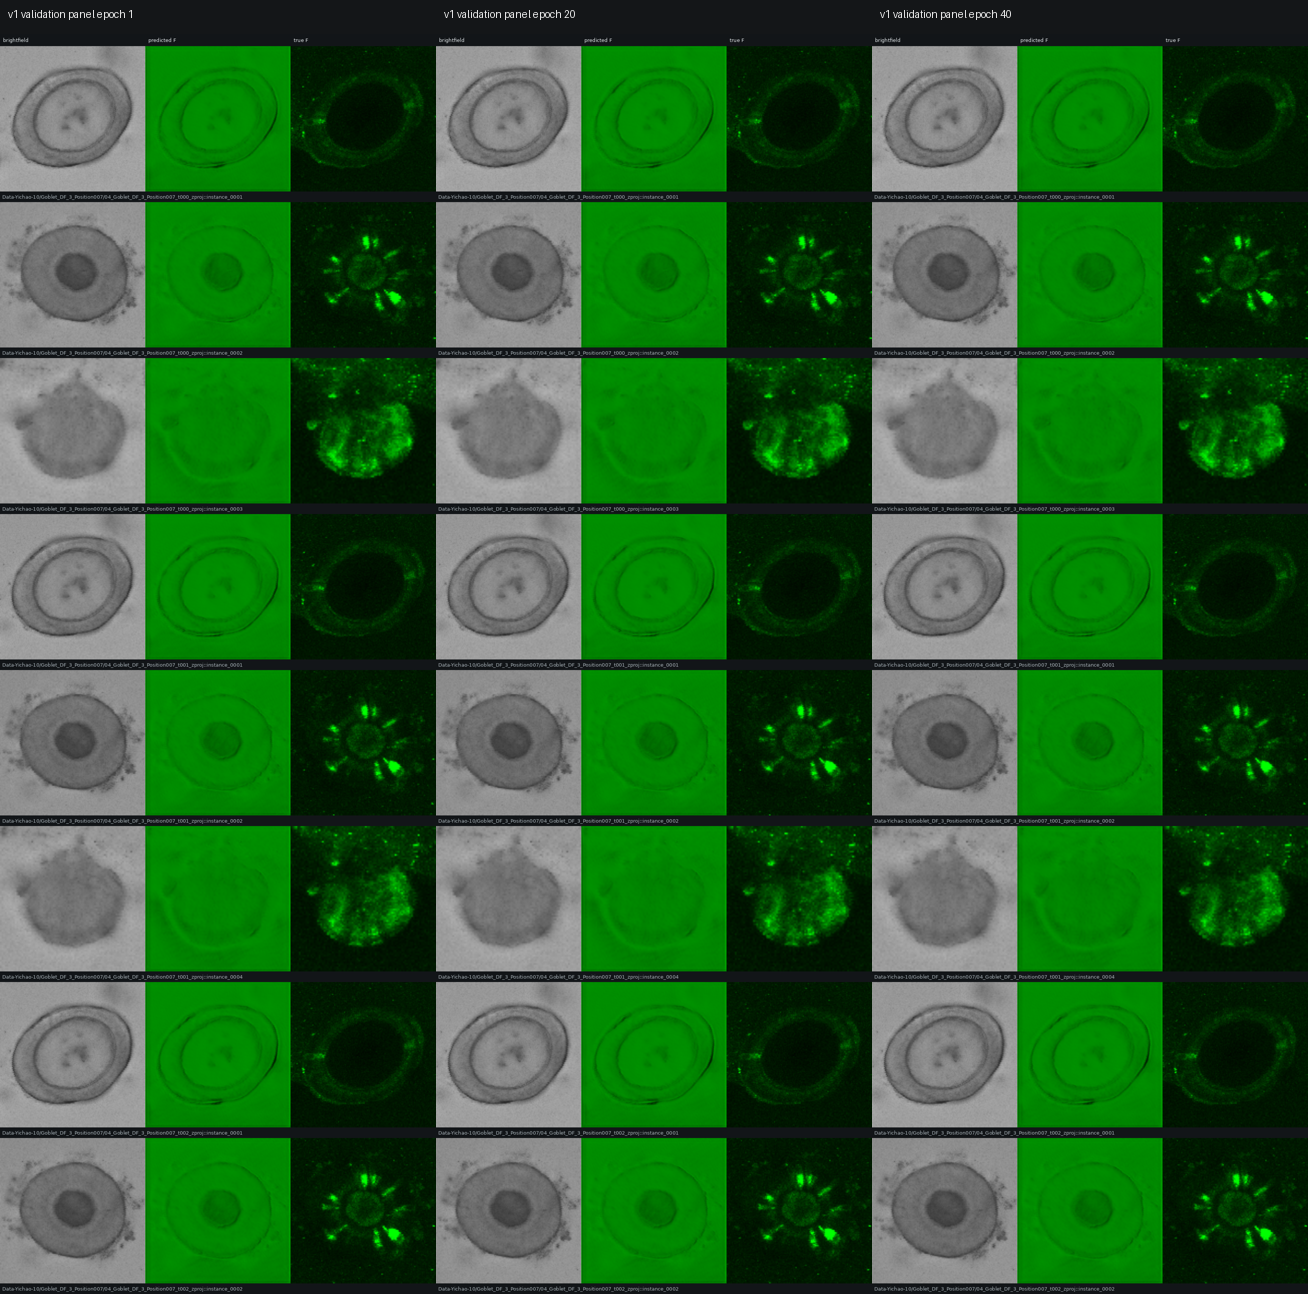
\includegraphics[width=\linewidth]{figures/fig2_v1_panel_progression.png}
\caption{v1 validation panels at epochs 1, 20, and 40. The predicted fluorescence remains a broad green brightfield-like image instead of matching the sparse true fluorescence signal.}
\label{fig:v1-panels}
\end{figure}

\begin{figure}[H]
\centering
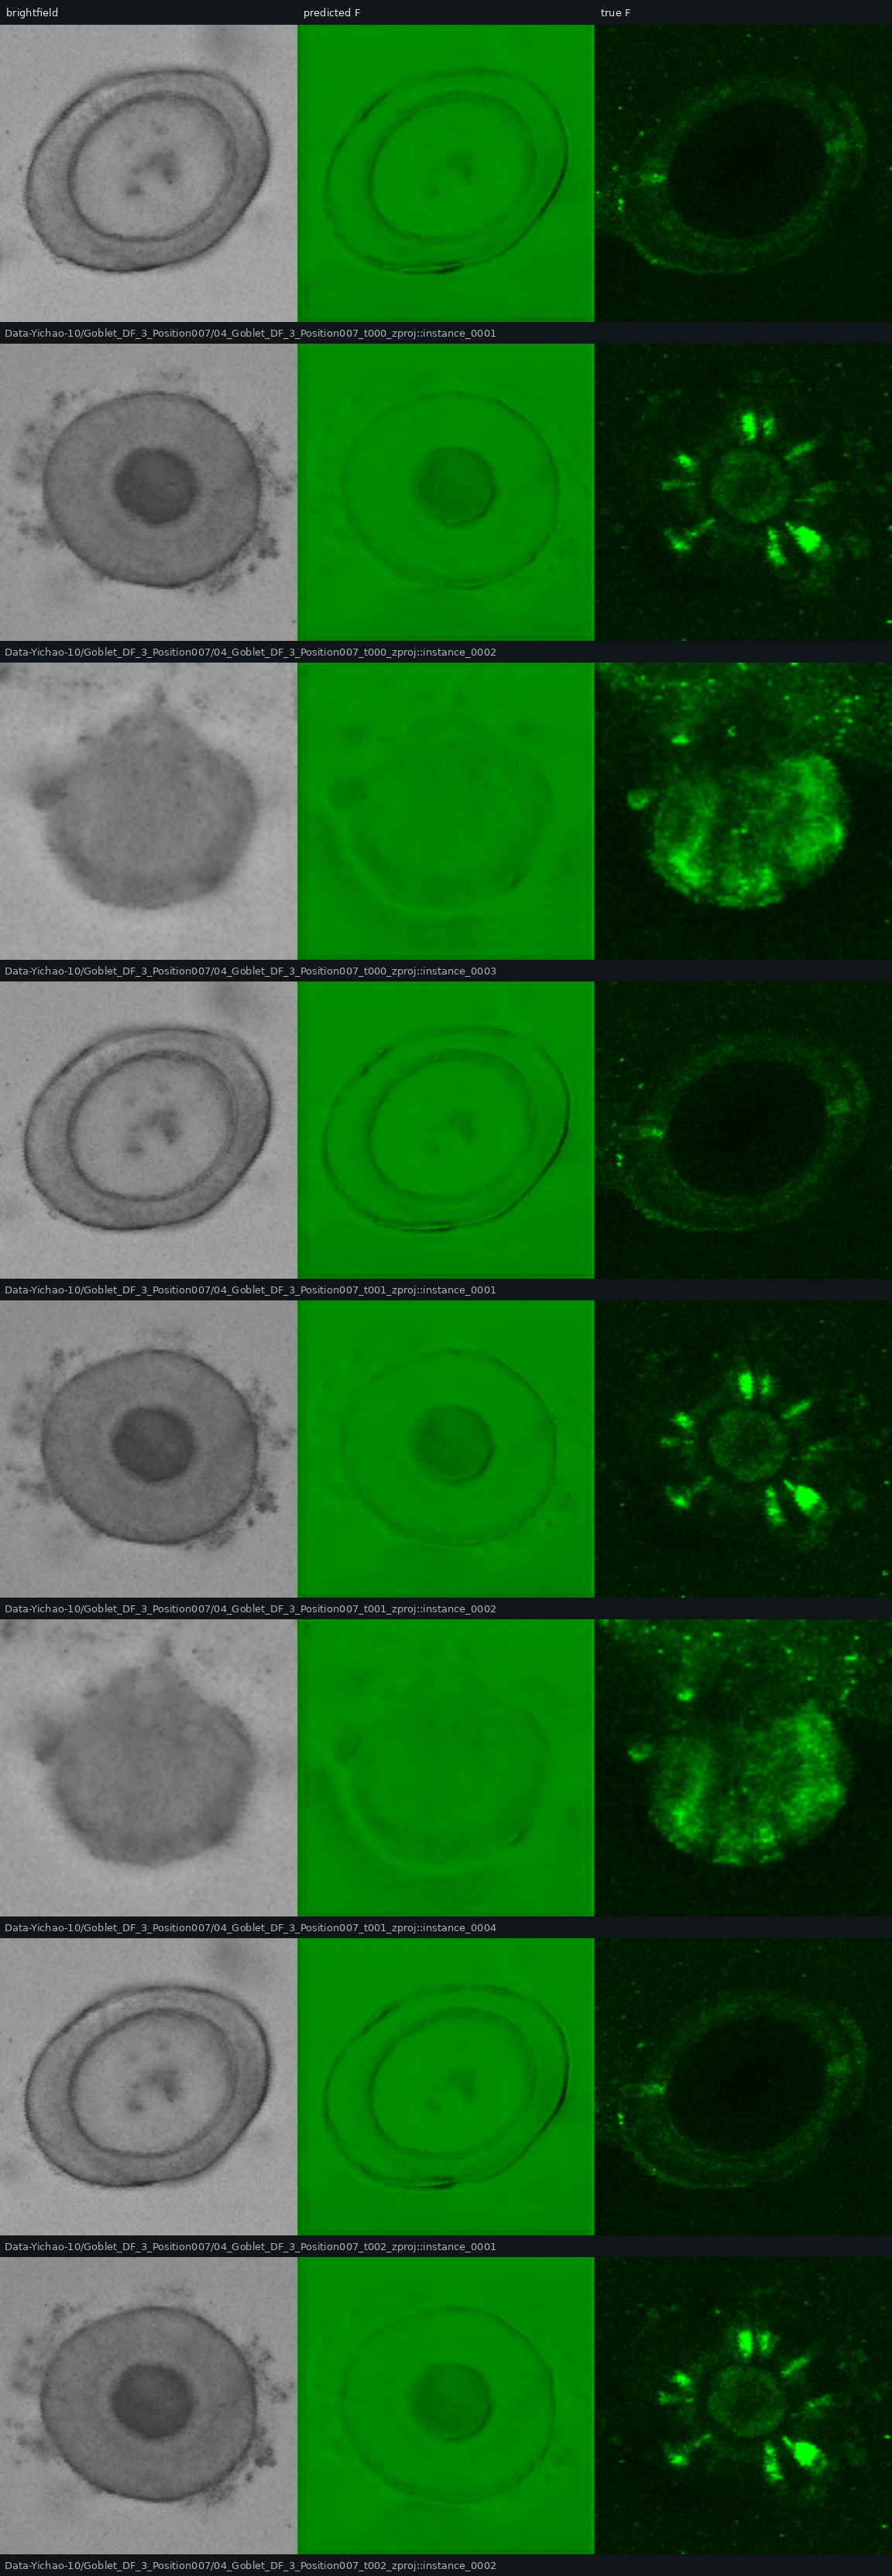
\includegraphics[height=0.82\textheight,keepaspectratio]{figures/fig3_v1_epoch20_panel.png}
\caption{v1 epoch 20 validation examples. Columns are brightfield input, predicted fluorescence, and true fluorescence. The prediction copies broad morphology and does not localize the true fluorescent structures.}
\label{fig:v1-epoch20}
\end{figure}

\section{Why v1 Did Not Work}

The v1 result should not be interpreted as ``needs 1000 epochs''. It failed for identifiable technical reasons:

\begin{enumerate}
\item \textbf{Low-threshold binary pixel target.} The loss converted fluorescence into a binary target using a low threshold. Many organoid pixels exceeded that threshold, so the model was rewarded for predicting broad green signal inside the organoid.
\item \textbf{Misleading signal recall/F1.} Because the prediction was above the low signal threshold nearly everywhere inside the mask, recall was almost 1.0 even though the visual prediction was wrong.
\item \textbf{Scalar auxiliary loss was too strong.} The scalar head was useful, but its loss weight was too large for a run whose main purpose is image reconstruction.
\item \textbf{Runtime instability.} The v1 tmux command used channels-last plus SiLU activations. The run stopped with \texttt{TypeError: silu() keywords must be strings}.
\item \textbf{Rare expression examples remain a data problem.} Image-level expression labels are imbalanced, so AUROC cannot be the main checkpoint-selection metric.
\end{enumerate}

\section{Correction Implemented}

The correction is committed in:

\begin{center}
\small
\texttt{8cbfb62 training: fix strong B2F loss and runtime}
\end{center}

Code paths:

\begin{itemize}
\item \path{/home/lachlan/ProjectsLFS/OrganoidAgent/differentiation_prediction/yichao_future_expression/train_b2f_strong.py}
\item \path{/home/lachlan/ProjectsLFS/OrganoidAgent/differentiation_prediction/yichao_future_expression/models.py}
\item \path{/home/lachlan/ProjectsLFS/OrganoidAgent/differentiation_prediction/yichao_future_expression/resume_strong_b2f_tmux.sh}
\item \path{/home/lachlan/ProjectsLFS/OrganoidAgent/references/Yichao/b2f_strong_training_strategy.md}
\end{itemize}

The important algorithmic changes are:

\begin{enumerate}
\item Replace SiLU with GELU in the strong B2F model.
\item Remove channels-last from the long-run tmux command.
\item Replace low-threshold binary fluorescence BCE with continuous target-intensity supervision.
\item Use Charbonnier intensity loss weighted by true fluorescence intensity.
\item Use soft BCE against the real fluorescence intensity target, not a binary mask.
\item Lower the scalar auxiliary weight so image reconstruction drives the model.
\item Raise the signal threshold used for diagnostic signal metrics from 0.08 to 0.25.
\end{enumerate}

Mathematically, v2 is now closer to:

\begin{equation}
\mathcal{L}_{\mathrm{image}}
=
\frac{\sum_i w_i \sqrt{(\hat{F}_i-F_i)^2+\epsilon^2}}{\sum_i w_i},
\quad
w_i = w_0 + M_i(1+\alpha F_i^{1.5}),
\end{equation}

with additional soft BCE, SSIM, edge, and small scalar auxiliary terms. This directly penalizes broad green predictions in dark regions while still emphasizing bright fluorescence.

\section{v2 Smoke Test}

\begin{figure}[H]
\centering
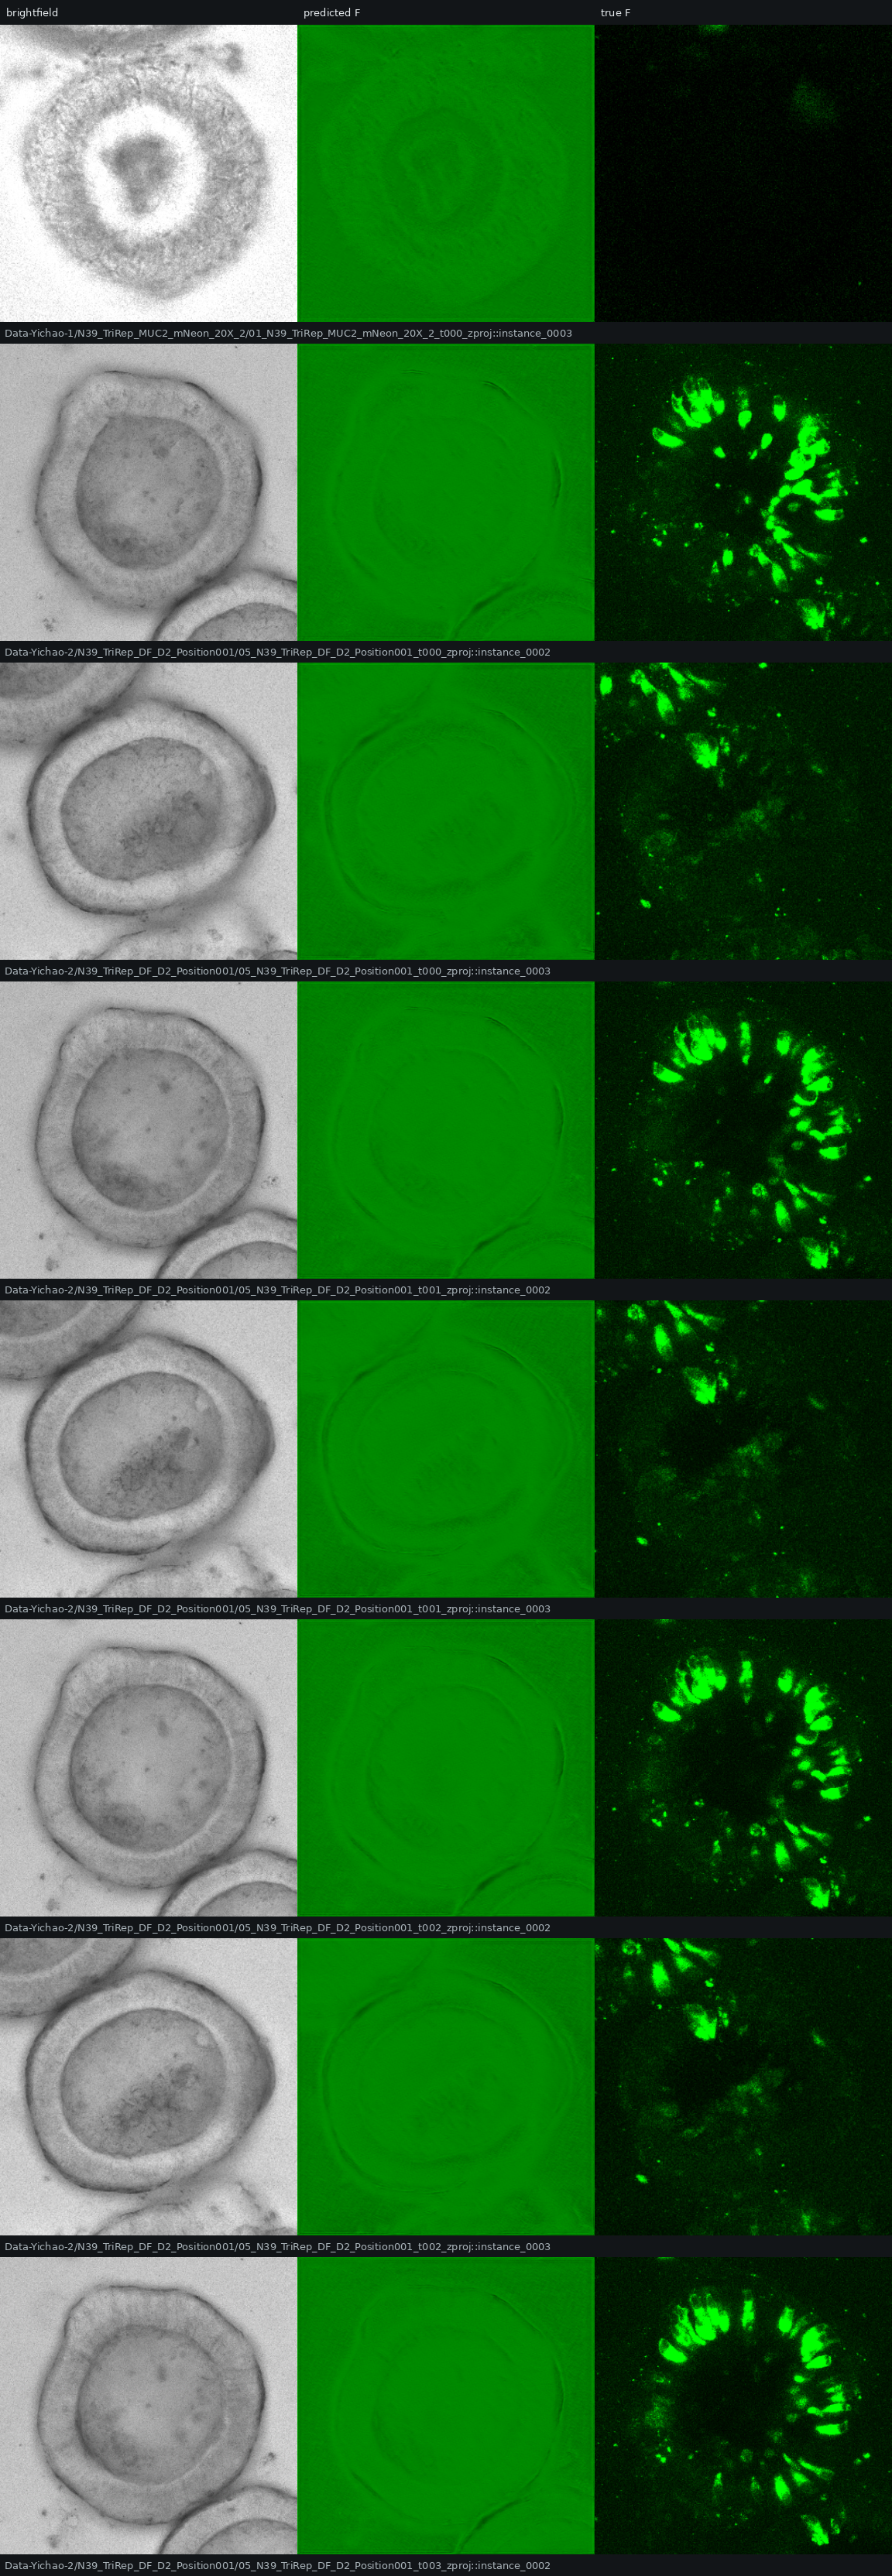
\includegraphics[height=0.82\textheight,keepaspectratio]{figures/fig4_v2_smoke_panel.png}
\caption{v2 384 px configuration smoke-test panel. This is only a one-epoch smoke test, so it is not a performance result. Its purpose is to confirm that the corrected model/loss runs and writes prediction panels.}
\label{fig:v2-smoke}
\end{figure}

\section{Success Criteria For The Active Run}

The active v2 run should be judged by the following, not by epoch count alone:

\begin{enumerate}
\item Validation panels should stop showing broad green brightfield-copy outputs.
\item \texttt{val\_masked\_mae} and \texttt{val\_signal\_mae} should decrease.
\item \texttt{val\_signal\_precision} should improve without recall staying trivially 1.0.
\item \texttt{val\_peak\_pearson} should become positive and increase.
\item The best checkpoint should be selected by reconstruction/signal quality, not rare expression AUROC.
\end{enumerate}

\section{Next Step}

Do not restart future prediction yet. The correct next step is to let v2 train long enough to inspect panels at epochs 20, 40, 60, and 100. If v2 starts producing visually plausible same-time fluorescence, then its encoder should be used to initialize the future model. If v2 remains broad/smooth, the next escalation should be a pix2pix-style adversarial/perceptual image loss and a cleaner expression-positive subset, not simply more epochs.

\end{document}
